\documentclass[a4paper]{article}

% Packages
\usepackage[margin = 1 in]{geometry}
\usepackage{fancyhdr}
\usepackage{lastpage}
\usepackage{ctex}
\usepackage[utf8]{inputenc} % Required for inputting international characters
\usepackage[english]{babel}
\usepackage[T1]{fontenc} % Output font encoding for international characters
\usepackage[sfdefault]{ClearSans} % Use the Clear Sans font (sans serif)
\usepackage{graphicx}
\usepackage{caption}
\usepackage{subcaption}
\usepackage{float}
\usepackage{amsmath}
\usepackage{amsfonts}
\usepackage{enumitem}
\usepackage{hyperref}
\usepackage{titlesec}
\usepackage{lipsum}
\usepackage{geometry}
\usepackage{tocloft} 

\pagestyle{fancy}
% Formatting
\geometry{margin=1in}
\setlength{\parindent}{0pt}
\setlength{\parskip}{1em}
\renewcommand{\baselinestretch}{1.5}
\renewcommand{\cftsecleader}{\cftdotfill{\cftdotsep}}
\rhead{\thepage}

% Title and Author
\title{\textbf{Challenges and Strategies for Sentiment Analysis of Irony and Humor in Social Media Based on Machine Learning}}
\author{Zijun Li}
\date{\today}

% Document
\begin{document}
\setlength{\parindent}{2em}

% Title Page
\maketitle
\thispagestyle{empty}

%% Abstract
\begin{abstract}
    Sentiment analysis of irony and humor in social media poses a formidable challenge owing to the complexity and context-dependency of such expressions. This report offers a comprehensive overview of diverse machine learning techniques utilized in the analysis of irony and humor, encompassing traditional machine learning algorithms and deep learning approaches. We explore the practical implementation of these techniques by examining specific examples and assess the challenges and future prospects of sentiment analysis concerning irony and humor in social media.
\end{abstract}

% Table of Contents
% \newpage
% \tableofcontents
% \thispagestyle{empty}

% Introduction
\newpage
\setcounter{page}{1}
\section{Introduction}

The growing popularity of social media platforms has made it increasingly essential to understand user sentiment through their text for various applications such as marketing, customer service, and opinion mining. Irony and humor are common in social media and present significant challenges for sentiment analysis due to their context-dependency, diverse forms, and complex language features.

As science and technology progress, artificial intelligence has gradually permeated from specialized domains to everyday life. According to the Verta Insights Study, among investment strategies for six different spending categories in 2022 and 2023, the AI innovation technology category remains the top priority, ranked as a priority by 54\% and 58\% of respondents, respectively. This demonstrates the significance of artificial intelligence technology in social development.

This report provides an overview of the challenges and strategies for sentiment analysis of irony and humor in social media using machine learning techniques. We begin by defining irony and humor, followed by an examination of various strategies and their practical implementations. Finally, we discuss the challenges and future directions for this area of research.

% irony and Humor in Sentiment Analysis
\section{The basic concepts of irony and humor sentiment analysis}

Prior to exploring machine learning methods for analyzing irony and humor in sentiment analysis, it is crucial to establish a clear understanding of the definitions of irony and humor. This will facilitate better classification and labeling of data for analysis.

\subsection{The concepts of Irony}

Irony is a rhetorical device that conveys a meaning that is opposite or different from its literal meaning. It is commonly used in literature, language, and everyday conversation to create humor, emphasize a point, or express subtle criticism. Irony can be categorized into several types, but two of the most common types are verbal irony and situational irony.

\begin{itemize}
    \item {\bf Verbal irony} Irony is a rhetorical device that communicates a meaning opposite or distinct from its literal meaning. Frequently employed in literature, language, and everyday conversation, irony creates humor, emphasizes points, or expresses subtle criticism. Irony can be categorized into several types, with verbal irony and situational irony being among the most common.
    \item {\bf Situational irony} arises when the opposite of what is expected transpires. Often utilized to create a dramatic effect, add depth to a story, or convey a moral lesson, situational irony features prominently in literature. For example, in Shakespeare's play Romeo and Juliet, the two lovers plan to elope and live happily ever after. However, a series of tragic events thwarts their plans, culminating in their untimely deaths. The situational irony in this story lies in the fact that their pursuit of happiness ultimately leads to their tragic demise. 
\end{itemize}

Both verbal and situational irony serve as essential tools in communication and storytelling. They can introduce humor, convey deeper meanings, and create memorable moments. By understanding these types of irony, we can appreciate and analyze the intricate ways language is employed for communication and entertainment.

\subsection{The concepts of Humor}

Humor is a multifaceted and subjective concept, often defined as a form of communication that elicits laughter and entertainment, typically prompted by unexpected or incongruous situations. There are numerous types of humor, ranging from slapstick and physical comedy to wit.

Humor can be verbal, visual, or physical. In this discussion, we will concentrate on verbal humor, which can be further classified into the following categories:

\begin{itemize}
\item {\bf Self-irony}: Referring to self-irony, frequently employed to defuse tense situations or alleviate embarrassment. Example:
\subitem\textit{"I hate it when I go to hug someone really sexy and my face smashes right into the mirror."}
\\Using self-irony to indicate that the "someone sexy" is the speaker.
\item {\bf Exaggeration/Hyperbole}: Utilizing extreme exaggeration to emphasize a point or add humor. Example:
\subitem\textit{"I'm so hungry, I could eat a horse!"}
\\Normally, a human cannot eat an entire horse. The extreme exaggeration is used to convey the speaker's intense hunger.
\item {\bf Phonetics Assisted}: Generating humor by manipulating phonetic and pronunciation features. The production of this humor usually depends on the syllables, rhythm, and intonation of the language. Example:
\subitem\textit{"I'm reading a book on the history of glue – I just can't seem to put it down."}
\\The double meaning of the phrase "put it down" is employed because it can refer to physically placing a book down and stopping reading a book.
\item {\bf Semantic Opposites}: Using words with opposite meanings to create a humorous effect. Example:
\subitem\textit{"I love sleeping, it's like being dead without the commitment."}
\\This example underscores the speaker's love for sleeping by using the contrasting idea of death without its finality.
\item {\bf Secondary Meaning}: A word or phrase with multiple meanings, used to create a humorous effect. Example:
\subitem\textit{"Why do we tell actors to 'break a leg'? Because every play has a cast."}
\\In this example, the phrase "break a leg" possesses a secondary meaning in the theater world as a way of wishing someone good luck before a performance, even though the literal meaning is negative.
\end{itemize}

Humor classification is crucial for recognizing and interpreting different types of humor, as each necessitates unique analysis methods. For example, self-irony serves to mitigate awkward situations, while exaggeration/hyperbole employs exaggeration for comedic effect. Phonetics assisted humor relies on playing with phonetics and pronunciation features, whereas semantic opposites utilize opposites for humorous impact. Secondary meaning capitalizes on multiple meanings of words or phrases to generate comedic effect. Familiarity with these diverse types of humor can enhance our ability to recognize and comprehend humor. Moreover, for sentiment analysis in natural language processing, identifying humor can improve the accuracy of emotion and semantic interpretation of text.

% Machine Learning-based Strategies for Sentiment Analysis of irony and Humor in Social Media
\section{Sentiment analysis strategy for irony and humor based on machine learning}

Sentiment analysis methods based on machine learning are typically categorized into traditional machine learning and deep learning approaches. In this section, we will explore traditional machine learning methods, such as Support Vector Machines (SVM), Decision Trees, Random Forests, and Naive Bayes Classifier, as well as deep learning models, including Convolutional Neural Networks (CNN), Recurrent Neural Networks (RNN), Transformers and so on. We will discuss how these techniques can be applied to sentiment analysis tasks related to irony and humor.

\subsection{Machine learning algorithms}

Machine learning algorithms, a subset of artificial intelligence, enable machines to learn and enhance their performance from experience without explicit programming. These algorithms are extensively employed in sentiment analysis, including the analysis of irony and humor.

In sentiment analysis of irony and humor, feature engineering is a prevalent approach where relevant features, such as sentiment words, part-of-speech tags, and syntactic patterns, are identified and employed to train the classifier. For instance, detecting the presence of positive or negative sentiment words in a text can aid in classifying humor, while recognizing ironic expressions like understatement or overstatement can be utilized to classify irony.

Another approach involves ensemble methods, which integrate multiple classifiers to enhance the accuracy of the analysis. For example, combining decision trees and support vector machines (SVMs) could be employed to classify text as humorous or non-humorous. Ensemble methods have demonstrated improved performance in sentiment analysis of irony and humor compared to individual classifiers.

\subsubsection{Support Vector Machines, SVM}

SVM is a supervised learning algorithm applied to classification and regression problems. The fundamental principle of SVM involves dividing the dataset into different categories by identifying an optimal hyperplane. For binary classification, SVM seeks a hyperplane during training that maximizes the boundary between two distinct categories, thereby partitioning the data. If the dataset is linearly separable, SVM will identify a unique hyperplane separating the data into two classes. If the dataset is not linearly separable, SVM employs a technique called kernel function to transform the data from the original space to a higher-dimensional space, rendering the data linearly separable in this new space.

\begin{figure}[H]
    \centering
    \begin{minipage}{0.48\textwidth}
      \centering
      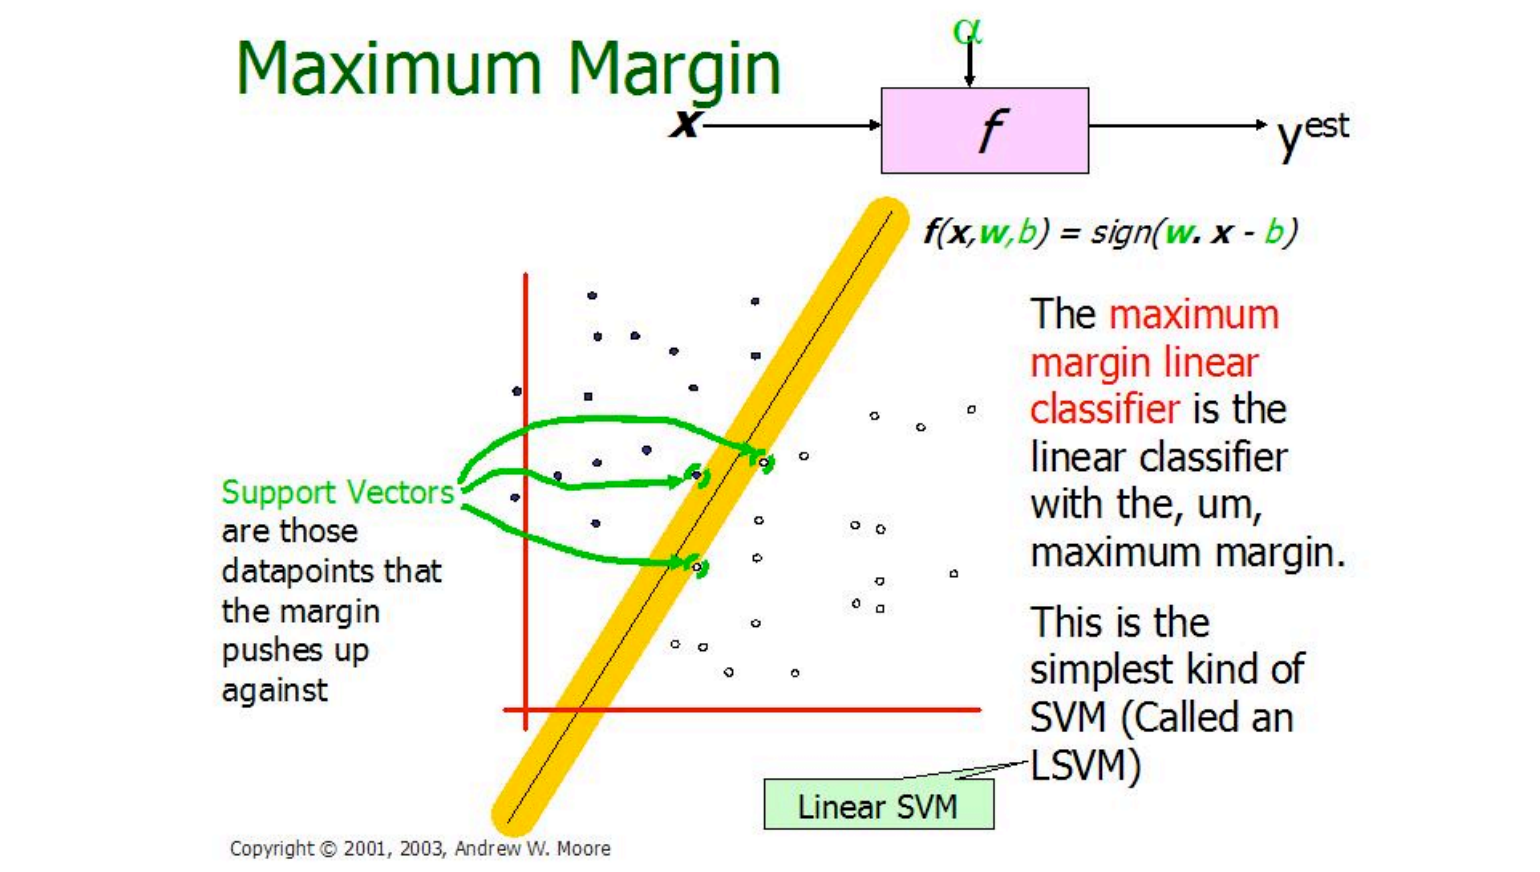
\includegraphics[width=\linewidth]{./images/SVM_Linear SVM.png}
      \caption{SVM: Linear SVM}
      \label{fig.SVM_Linear SVM[Illustration of Linear SVM. (Taken from Andrew W. Moore slides 2003)]}
    \end{minipage}\hfill
    \begin{minipage}{0.48\textwidth}
      \centering
      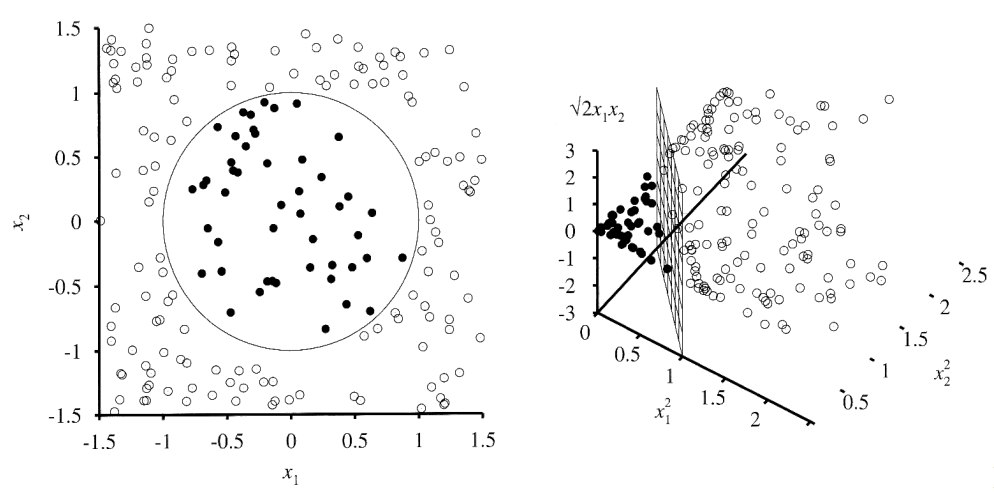
\includegraphics[width=\linewidth]{./images/SVM_High-dimensional_Space.png}
      \caption{SVM: Mapping data into a high-dimensional space}
      \label{fig.SVM_High-dimensional_Space[SVMTutorial]}
    \end{minipage}
  \end{figure}

SVM's advantage lies in its performance when handling high-dimensional data and achieving high-precision classification on smaller datasets. Additionally, SVM is robust, demonstrating a good tolerance for noise and outliers in the data.

It is worth noting that SVM requires selecting appropriate hyperparameters during training, such as regularization parameters and kernel function types. The choice of these hyperparameters may affect SVM's performance and thus needs proper tuning and validation.

For specific sentiment analysis tasks, humor and irony can be considered unique emotional expressions, corresponding to two emotional labels, such as "positive" and "negative". During training, existing humorous and satirical texts are labeled as "positive", while other texts are labeled as "negative", training a binary classifier. When using the trained model for sentiment analysis on new text, if the classifier judges it as "positive", the text can be considered to express humorous or ironic emotions.

Assume we have a dataset containing humorous and non-humorous sentences. We can represent each sentence as a feature vector, where each feature denotes a linguistic characteristic in that sentence, such as vocabulary, grammatical structure, or emotion.

For example, we can use a bag-of-words model to represent each sentence as a vector, where each dimension corresponds to a word's frequency in that sentence. For the sentence "What a nice day", this vector might be [0, 1, 0, 1, 0, 0, ...], where the second and fourth dimensions correspond to the frequencies of "day" and "nice".

For each sentence in the training set, we also need to assign it a class label, such as "humor" or "non-humor". This will be the target variable for our SVM. We can fit this dataset using the SVM algorithm to find the best hyperplane to segment humorous and non-humorous sentences.

For a new unknown sentence, we can represent it as a feature vector, and then use the trained SVM model to predict whether it is humorous or not.

\subsubsection{Decision Trees \& Random Forests}

A decision tree is a tree-structured classification algorithm that partitions the dataset, with each internal node representing a feature and each leaf node representing a category. The decision tree is built recursively, selecting each node based on a specific characteristic, typically using information gain or the Gini index. Information gain measures a feature's importance for classification, while the Gini index measures the purity of samples.

During the decision tree's classification process, starting from the root node, input samples are categorized according to the characteristics represented by each node, then assigned to corresponding child nodes until reaching the leaf nodes. Each leaf node represents a category, and the sample is ultimately assigned to a specific leaf node, which constitutes the sample's classification result.

\begin{figure}[H]
    \centering
    \begin{minipage}{0.48\textwidth}
      \centering
      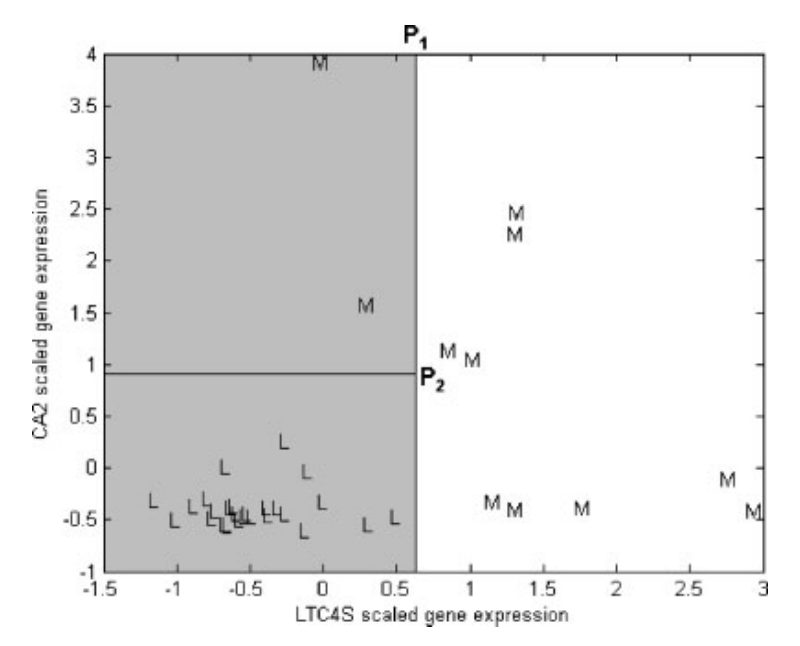
\includegraphics[width=\linewidth]{./images/Decision tree-Recursively-partitioned feature space.png}
      \caption{Decision tree: Recursively-partitioned feature space (features 1 and 2) of $X_T$.}
      \label{fig.Decision tree-data[An introduction to decision tree modeling]}
    \end{minipage}\hfill
    \begin{minipage}{0.48\textwidth}
      \centering
      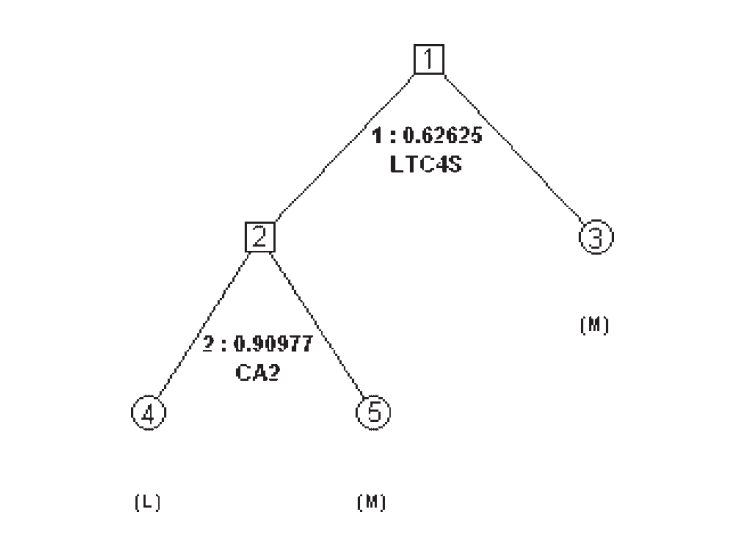
\includegraphics[width=\linewidth]{./images/Decision tree.png}
      \caption{Decision tree: Decision tree corresponding to the partitioned feature space in Figure 3.}
      \label{fig.Decision tree[An introduction to decision tree modeling]}
    \end{minipage}
\end{figure}

To prevent overfitting, the decision tree undergoes continuous pruning during training based on the training data. Pruning is generally divided into two methods: pre-pruning and post-pruning. Pre-pruning limits each node's division during tree construction to avoid overfitting, while post-pruning trims a complete tree after establishment to reduce overfitting.

Random Forests is an ensemble learning method that enhances classification or regression accuracy by constructing multiple decision trees. Each decision tree is obtained by randomly subsampling the training data and training with a random subset of features. At testing time, each decision tree classifies or regresses the input data, and the results from all decision trees are integrated to produce a final prediction.

In the random forest algorithm, we need to gather a collection of humorous or sarcastic text data and label it (e.g., humorous or non-humorous, sarcastic or not). This data is then split into training and testing sets.

We use the random forest algorithm to train the training set, generating multiple decision trees. At each decision tree node, we select a feature to classify and divide the dataset into two subsets. This process repeats until specific conditions are met.

On the test set, we use the generated decision tree for classification, counting the classification accuracy, and optimizing the algorithm.

For sentiment analysis of humor and irony, we can utilize linguistic features in the text data (such as word count, word frequency, part of speech, etc.) as features, and classify using the random forest algorithm to identify humorous and ironic expressions in the text.

\subsubsection{Naive Bayes Classifier}

The Naive Bayes classifier is a machine learning algorithm based on Bayes' theorem, which assumes feature independence, meaning the values of each feature under a given category are independent.

Specifically, the Naive Bayes classifier transforms a text data sentiment classification problem into a conditional probability calculation. Given text data $D$, the probability $P(c|D)$ of it belonging to a certain sentiment category $c$ must be calculated. According to Bayes' theorem, $P(c|D)$ can be expressed as:

$$P(c|D)=\dfrac{P(D|c)P(c)}{P(D)}$$

Here, $P(D|c)$ denotes the probability of text data $D$ occurring under the given emotion category $c$; $P(c)$ represents the probability of emotion category $c$ occurring; and $P(D)$ is the probability of text data $D$ occurring. As $P(D)$ is identical for all sentiment categories, it can be disregarded.

The Naive Bayes classifier presumes that for a given class $c$, the values of each feature $x_i$ are independent. Thus, the conditional probability $P(D|c)$ can be expressed as:

$$P(D|c)=P(x_1|c) \times P(x_2|c) \times ... \times P(x_n|c)$$

Here, $x_1, x_2, ..., x_n$ represent the features of text data $D$, and $n$ is the number of features.

For sentiment analysis of humor and irony, linguistic features in the text data (such as word count, word frequency, part of speech, etc.) can be used as features. The Naive Bayes classifier algorithm can classify and identify humorous and ironic expressions in the text.

For instance, given a dataset of labeled sentences as humorous or non-humorous, each sentence can be represented as a feature vector using a bag-of-words model. The Naive Bayes classifier can be trained on this data by calculating the conditional probabilities of each word given the class label. Once the model is trained, it can predict the humor class of new sentences based on their word frequencies.

\subsubsection{Summary}

\begin{table}[ht]
    \centering
    \renewcommand{\arraystretch}{1.2}
    \resizebox{\textwidth}{!}{%
    \footnotesize
    \begin{tabular}{|p{3cm}|p{5cm}|p{5cm}|p{2cm}|p{3cm}|}
    \hline
    Model & Advantages & Disadvantages & Use Cases & Applications \\ \hline
    Support Vector Machines & Effective in high-dimensional spaces, \newline robust to outliers, \newline maximizes margin between classes & May not perform well on large datasets, \newline sensitive to choice of kernel & Text classification, \newline image classification, \newline regression & Sentiment analysis, \newline handwriting recognition, \newline bioinformatics \\ \hline
    Decision Trees \newline and Random Forests & Easy to interpret, \newline can handle mixed data types, \newline scalable to large datasets (Random Forests) & May be prone to overfitting (Decision Trees), \newline can be complex and computationally expensive (Random Forests) & Classification, \newline regression, \newline feature selection & Customer segmentation, \newline fraud detection, \newline medical diagnosis \\ \hline
    Naive Bayes Classifier & Easy to implement, \newline computationally efficient, \newline handles missing data & Assumes feature independence, \newline may not perform well when features are correlated & Text classification, \newline spam filtering, \newline sentiment analysis & Sentiment analysis, \newline document classification, \newline spam detection \\ \hline
    \end{tabular}%
    }
    \resizebox{\textwidth}{!}{%
    \footnotesize
    \begin{tabular}{|p{3cm}|p{7cm}|p{8cm}|}
    \hline
    Model & Input Data & Key Formulas \\ \hline
    Support Vector Machines & Input: $X \in \mathbb{R}^{n \times d}$ (feature matrix), \newline Labels: $y \in {-1, 1}^n$ (class labels) & Decision function: $f(x) = w^T \phi(x) + b$,\newline Objective: $\min_{w, b} \frac{1}{2} |w|^2 + C \sum_{i=1}^n \xi_i$, \newline Constraint: $y_i (w^T \phi(x_i) + b) \geq 1 - \xi_i, \xi_i \geq 0$ \\ \hline
    Decision Trees \newline and Random Forests & Input: $X \in \mathbb{R}^{n \times d}$ (feature matrix), \newline Labels: $y \in \mathbb{R}^n$ (class labels or continuous target) & Decision Tree: $y = f(x)$,\newline Random Forest: $y = \frac{1}{B} \sum_{b=1}^B f_b(x)$, \newline where $f_b(x)$ is a decision tree \\ \hline
    Naive Bayes Classifier & Input: $X \in \mathbb{R}^{n \times d}$ (feature matrix), \newline Labels: $y \in \mathbb{R}^n$ (class labels) & Conditional probability: $P(c|D) = \frac{P(D|c) P(c)}{P(D)}$, \newline Naive assumption: $P(D|c) = P(x_1|c) \times P(x_2|c) \times \cdots \times P(x_n|c)$ \\ \hline
\end{tabular}%
}
\end{table}

\subsection{Deep learning algorithm}

Deep learning algorithms have demonstrated considerable potential in numerous natural language processing tasks, encompassing sentiment analysis of irony and humor. This section explores prominent deep learning methods, including Convolutional Neural Networks (CNNs), Recurrent Neural Networks (RNNs), Long Short-Term Memory (LSTM) networks, and Transformers, and their applications in irony and humor analysis tasks.

\subsubsection{Convolutional Neural Networks (CNNs)}

Although CNNs are predominantly utilized in image processing, they can also be employed for text classification tasks, including irony and humor analysis. They operate by applying convolutional filters to extract features from text and pooling layers to diminish the dimensionality of the extracted features.

The application of CNNs in humor and irony sentiment analysis hinges on convolution and pooling operations. Convolution operations capture local features in the text, while pooling operations reduce feature dimensions and enhance feature robustness. CNNs accept text input as a matrix, convolve it with multiple convolution kernels, and then use pooling operations for feature extraction and dimensionality reduction. Ultimately, a fully connected layer classifies the features.

\begin{figure}[H]
    \centering
    \begin{minipage}{0.48\textwidth}
      \centering
      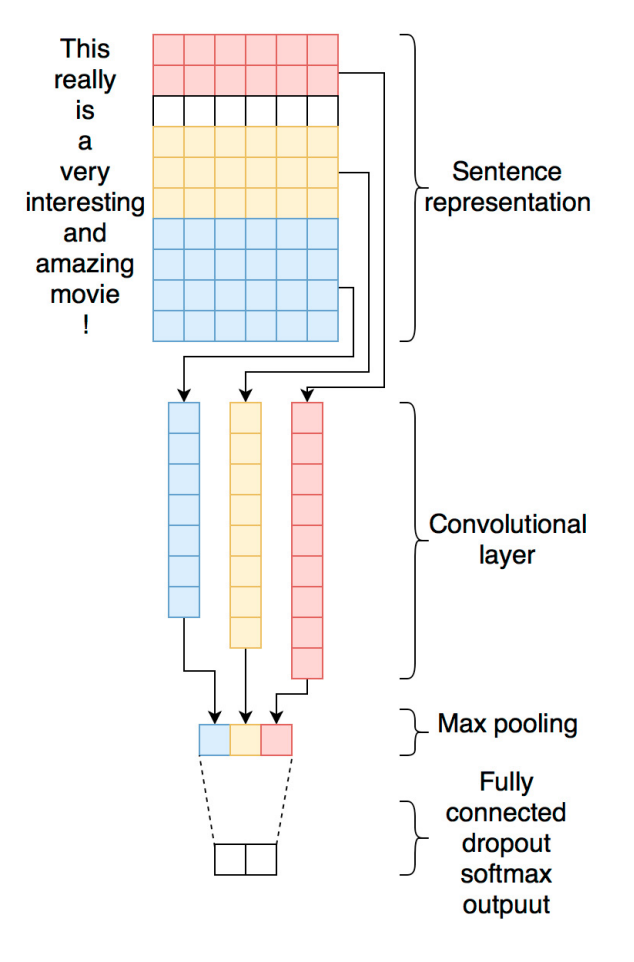
\includegraphics[width=\linewidth]{./images/CNN_architecture.png}
      \caption{CNN: Example architecture}
      \label{fig.CNN[CNN for situations understanding based on sentiment analysis of twitter data]}
    \end{minipage}\hfill
    \begin{minipage}{0.48\textwidth}
        The training process of CNNs entails the following steps:
        \begin{enumerate}
            \item Input layer: The input layer receives the text data for analysis.
            \item Convolutional layer: This layer applies a set of filters to the input data to detect specific features, such as word sequences, patterns, and structures.
            \item Pooling layer: The pooling layer downsamples the activation layer's output by summarizing the information in neighboring activations.
            \item Fully connected layer: This layer takes the pooling layer's output and applies a set of weights to generate a final output.
            \item Output layer: The output layer yields a probability distribution over possible sentiment labels (e.g., positive, negative, ironic, humorous).
        \end{enumerate}
    \end{minipage}
\end{figure}

In humor and irony sentiment analysis, CNNs typically receive text data input, such as phrases, sentences, or paragraphs. CNNs can autonomously learn to extract features from input text and utilize these features for sentiment classification. For instance, CNNs can automatically capture features like vocabulary and syntax to better comprehend the meaning of humorous and sarcastic expressions.

\subsubsection{Recurrent Neural Networks (RNNs)}

Recurrent Neural Networks (RNNs) constitute another deep learning algorithm suitable for humor and irony sentiment analysis. RNNs excel at analyzing sequential data, crucial for comprehending the context of humorous or ironic statements.

\begin{figure}[H]
    \centering
    \begin{minipage}{0.48\textwidth}
        \centering
        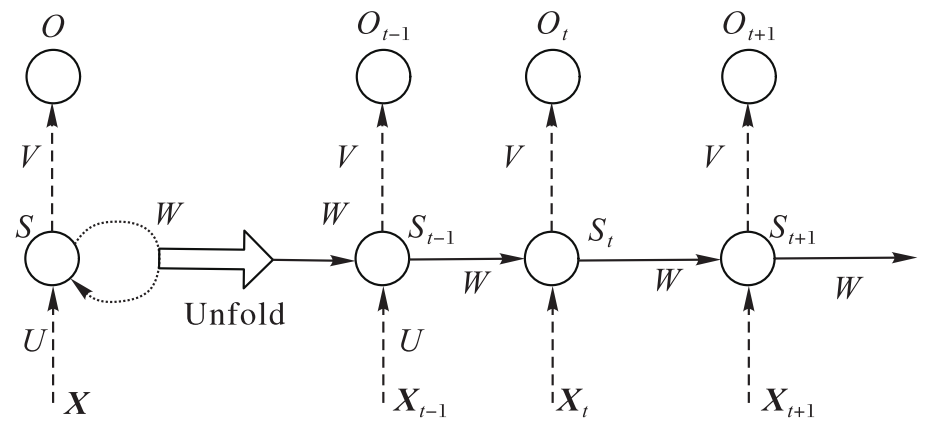
\includegraphics[width=1\textwidth]{./images/RNN_architecture.png}
        \caption{RNN: Example architecture}
        \label{fig.RNN[Review of applications of natural language processing in text sentiment analysis]}
    \end{minipage}\hfill
    \begin{minipage}{0.48\textwidth}
        The fundamental principle of RNNs involves using the output from a previous time step as input to the current time step, enabling the network to maintain a form of memory for previous inputs. This feature is especially beneficial for analyzing text sequences, where a word or phrase's meaning may rely on the context of preceding text.
    \end{minipage}
\end{figure}

Within the realm of humor and irony analysis, RNNs can be trained on extensive datasets of text labeled with humor or irony, subsequently learning to recognize patterns and dependencies in the data. These models can classify new text as humorous or ironic based on the patterns learned from the training data.

A significant application of RNNs in humor and irony analysis involves generating new text that is humorous or ironic. By training an RNN on a dataset of humorous or ironic text, the model can learn to generate new text that mirrors the style and tone.

\paragraph{Long Short-Term Memory (LSTM)}

Long Short-Term Memory (LSTM) represents a specialized RNN model designed for processing sequential data and has gained widespread use in irony and humor sentiment analysis.

\begin{figure}[H]
    \centering
    \begin{minipage}{0.48\textwidth}
        \centering
        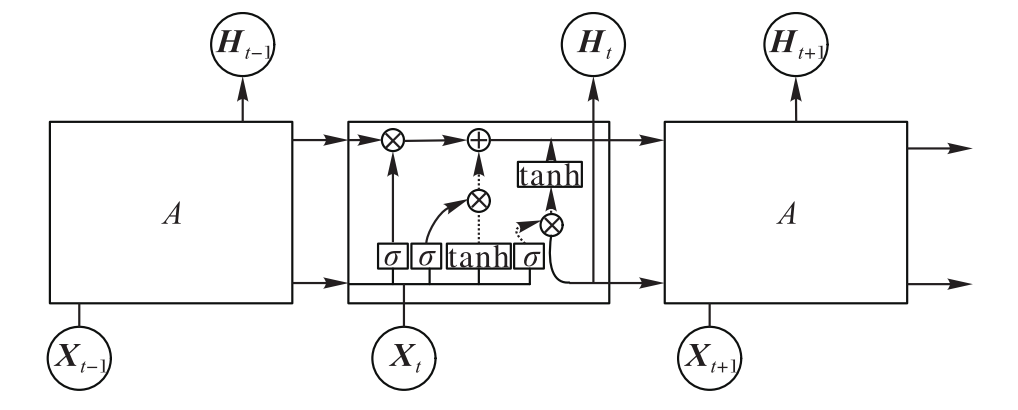
\includegraphics[width=1\textwidth]{./images/LSTM_architecture.png}
        \caption{LSTM: Example architecture}
        \label{fig.LSTM[Review of applications of natural language processing in text sentiment analysis]}
    \end{minipage}\hfill
    \begin{minipage}{0.48\textwidth}
        In contrast to traditional RNN models, LSTM incorporates three gate mechanisms: input, forget, and output gates. These gates control the influence of information passed from previous moments and current moment input on subsequent moments. This mechanism effectively addresses the vanishing gradient problem associated with long sequence data, thereby enhancing the model's performance.
    \end{minipage}
\end{figure}

In humor and irony sentiment analysis, LSTMs frequently model text sequences to capture contextual and semantic information within language. By learning long-term dependencies, LSTMs gain a better understanding of implicit semantics and logic in humor and irony, leading to improved sentiment analysis.

LSTM models typically require extensive data for training to achieve optimal performance. During the training process, the backpropagation algorithm updates the model's parameters, while techniques such as cross-validation evaluate the model's performance and generalization capabilities. Ultimately, the trained model performs sentiment analysis on new text data, classifying and recognizing humor and irony.

\paragraph{AttBiLSTM (Attention-based Bidirectional Long Short-Term Memory)}

AttBiLSTM (Attention-based Bidirectional Long Short-Term Memory) extends the LSTM model by incorporating an additional attention mechanism and bidirectionality.

\begin{figure}[H]
    \centering
    \begin{minipage}{0.48\textwidth}
        \centering
        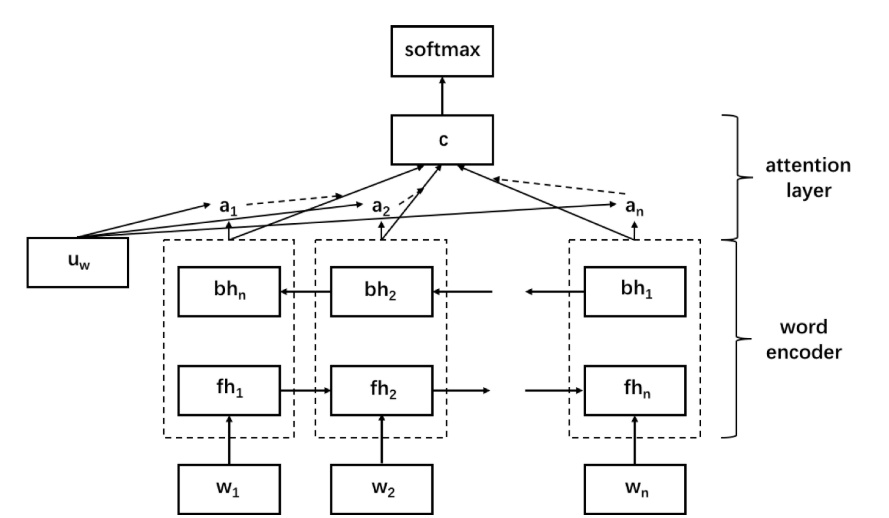
\includegraphics[width=1\textwidth]{./images/AttBiLSTM_architecture.png}
        \caption{AttBiLSTM: Example architecture}
        \label{fig.AttBiLSTM[HEMOS: A novel deep learning-based fine-grained humor detecting method for sentiment analysis of social media]}
    \end{minipage}\hfill
    \begin{minipage}{0.48\textwidth}
        In AttBiLSTM, a reverse LSTM processes the reverse part of the sequence at each time step, in addition to the forward LSTM. Furthermore, AttBiLSTM employs an attention mechanism to calculate the importance of each time step in the sequence, assigning importance to the corresponding hidden state to better capture key information within the sequence.
    \end{minipage}
\end{figure}

Compared to LSTM, AttBiLSTM offers superior sequence modeling and expressive capabilities, handles long sequences more effectively, and demonstrates higher performance in numerous natural language processing tasks.

\subsubsection{Transformers}

Transformers represent a neural network model based on the self-attention mechanism, originally proposed by Google. The core concept involves acquiring a comprehensive feature representation of the input sequence by executing self-attention weighted aggregation on the features of all positions within the input sequence.

Transformers generally comprise two stages: pre-training and fine-tuning. During the pre-training stage, the model learns to represent text data from a vast text corpus. In the fine-tuning stage, the model undergoes refinement on specific humor and irony datasets, enhancing its sentiment analysis capabilities for humor and irony. Distinct from traditional RNNs and CNNs, Transformers consider the semantics of the entire sentence when processing text, resulting in superior performance for humor and irony that require an understanding of contextual language forms.

\subsubsection{Summary}

\begin{table}[ht]
    \centering
    \renewcommand{\arraystretch}{1.2}
    \resizebox{\textwidth}{!}{%
    \footnotesize
    \begin{tabular}{|p{1.5cm}|p{5cm}|p{5cm}|p{3cm}|p{3cm}|}
        \hline
        Model & Advantages & Disadvantages & Use Cases & Applications \\ \hline
        CNN & Good at capturing local dependencies, \newline efficient computation for parallel processing & May not capture long-term dependencies, \newline not suitable for variable-length input & Text classification, \newline object recognition, \newline image processing & Sentiment analysis, \newline image classification, \newline speech recognition \\ \hline
        RNN & Can handle sequential data, \newline can capture long-term dependencies & May suffer from vanishing/exploding gradients, \newline computationally expensive & Language modeling, \newline speech recognition, \newline machine translation & Text generation, \newline speech synthesis, \newline handwriting recognition \\ \hline
        LSTM & Addresses vanishing/exploding gradient problem, \newline can capture long-term dependencies & Computationally expensive, \newline not suitable for parallel processing & Speech recognition, \newline machine translation, \newline handwriting recognition & Text generation, \newline speech synthesis, \newline video processing \\ \hline
        AttBiLSTM & Handles sequential data with attention mechanism, \newline captures both local and global dependencies & Computationally expensive, \newline may require large amounts of training data & Sentiment analysis, \newline language modeling, \newline machine translation & Text classification, \newline sentiment analysis, \newline chatbots \\ \hline
        Transformer & Enables parallel processing, \newline can handle long-term dependencies & May require a large amount of training data, \newline less effective for real-time sequential data & Machine translation, \newline language modeling, \newline text generation & Chatbots, \newline text classification, \newline sentiment analysis \\ \hline
    \end{tabular}%
    }
    \resizebox{\textwidth}{!}{%
    \footnotesize
    \begin{tabular}{|p{1.5cm}|p{10cm}|p{6cm}|}
        \hline
        Model & Input Data & Key Formulas \\ \hline
        CNN & Input: $X \in \mathbb{R}^{W \times H \times C}$ (image or time-series data),\newline Weights: $W \in \mathbb{R}^{w \times h \times C \times N}$ (convolutional kernel) & Convolution: $Y_{i} = f(X * W_{i} + b_{i})$ \\ \hline
        RNN & Input: $x_t \in \mathbb{R}^n$ (input at time step $t$),\newline Hidden state: $h_t \in \mathbb{R}^m$ (hidden state at time step $t$) & $h_t = f(W_{hh}h_{t-1} + W_{xh}x_t + b_h)$ \\ \hline
        LSTM & Input: $x_t \in \mathbb{R}^n$ (input at time step $t$),\newline Hidden state: $h_t \in \mathbb{R}^m$ (hidden state at time step $t$),\newline Cell state: $c_t \in \mathbb{R}^m$ (cell state at time step $t$) & $\begin{aligned}
            f_t &= \sigma(W_f[h_{t-1}, x_t] + b_f) \\
            i_t &= \sigma(W_i[h_{t-1}, x_t] + b_i) \\
            \tilde{c}_t &= \tanh(W_c[h_{t-1}, x_t] + b_c) \\
            c_t &= f_t \odot c_{t-1} + i_t \odot \tilde{c}_t \\
            o_t &= \sigma(W_o[h_{t-1}, x_t] + b_o) \\
            h_t &= o_t \odot \tanh(c_t)
        \end{aligned}$ \\ \hline
        AttBiLSTM & Input: $x_t \in \mathbb{R}^n$ (input at time step $t$),\newline Hidden state: $h_t \in \mathbb{R}^m$ (hidden state at time step $t$),\newline Attention weights: $\alpha_{ij}$ (attention weight for input $j$ at time step $i$) & $\begin{aligned}
            h_t^f &= \text{LSTM}_f(x_t, h_{t-1}^f) \\
            h_t^b &= \text{LSTM}_b(x_t, h_{t+1}^b) \\
            e_{ij} &= \text{score}(h_i^f, h_j^b) \\
            \alpha_{ij} &= \frac{\exp(e_{ij})}{\sum_{k=1}^T \exp(e_{ik})} \\
            c_i &= \sum_{j=1}^T \alpha_{ij} h_j^b \\
            h_i &= \text{tanh}(W_c[h_i^f; c_i]) \\
            \end{aligned}$ \\
            \hline
            Transformer & Input: $x \in \mathbb{R}^{T \times d_{\text{model}}}$ (sequence of embeddings),\newline Key, Query, Value: $K, Q, V \in \mathbb{R}^{T \times d_k}$ & $\begin{aligned}
            Z &= \text{Self-Attention}(Q, K, V) \\
            Z &= \text{LayerNorm}(x + Z) \\
            F &= \text{FeedForward}(Z) \\
            F &= \text{LayerNorm}(Z + F)\\
        \end{aligned}$ \\
        \hline
    \end{tabular}%
    }
\end{table}

\section{Actual case analysis}

\paragraph{HEMOS: A Novel Deep Learning-Based Fine-Grained Humor Detection Method for Sentiment Analysis of Social Media}

In a study conducted by Da Li, Rafal Rzepka, Michal Ptaszynski, and Kenji Araki, the researchers employed both lexicons and an \textbf{AttBiLSTM recurrent neural network} for sentiment analysis of Chinese social media, resulting in the creation of the HEMOS system.

\begin{figure}[H]
    \centering
    \begin{minipage}{0.48\textwidth}
        \centering
        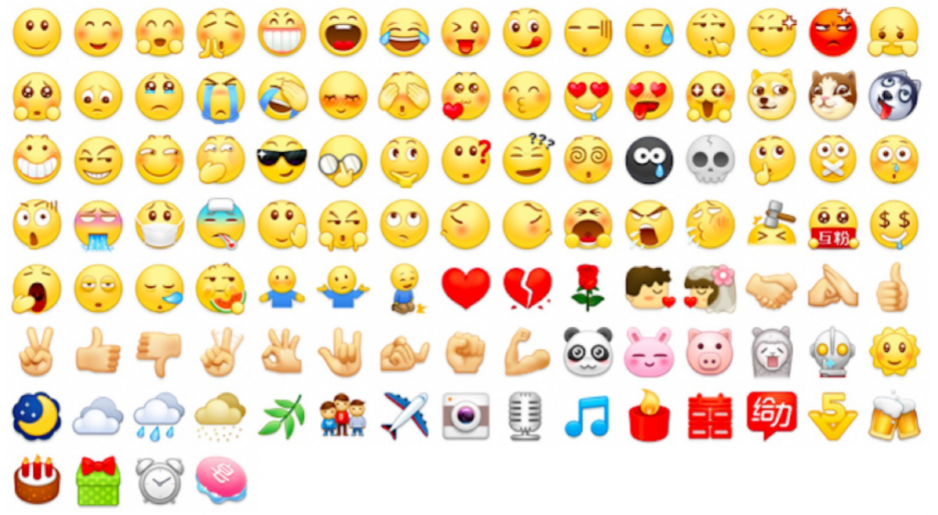
\includegraphics[width=1\textwidth]{./images/108_Weibo_emojis.png}
        \caption{109 Weibo emojis that can be transformed into Chinese character tags}
        \label{fig.109 Weibo emojis that can be transformed into Chinese character tags.[HEMOS: A Novel Deep Learning-Based Fine-Grained Humor Detection Method for Sentiment Analysis of Social Media]}
    \end{minipage}\hfill
    \begin{minipage}{0.48\textwidth}
        Since emotions are often expressed through body language, and in social networks, this nonverbal communication can be partially mimicked by employing emojis and slang. The researchers combined emoticons, slang, and text to analyze whether Weibo action comments contained humor.
    \end{minipage}
\end{figure}

Based on these emojis and slang, various meanings were assigned to different emojis and slang as one criterion for assessing humor. This approach facilitated a more nuanced understanding of the content analyzed and enhanced the accuracy of sentiment analysis.

The authors conducted research on sentiment analysis of Chinese social media, specifically focusing on detecting irony and humor in Weibo posts. They crawled a vast dataset of 7.6 million Weibo posts, filtered out images and videos, and trained word embeddings using the word2vec model. Additionally, they incorporated Chinese Internet slang and emoji lexicons into the dictionary of Jieba, a Chinese text segmentation package, to improve the accuracy of the text preprocessing stage.

To train their proposed model, the researchers collected 4000 Weibo posts containing ambiguous emojis and requested three Chinese native speakers to annotate them using four category labels: positive, negative, optimistic humorous, and pessimistic humorous. The AttBiLSTM model was subsequently trained with 10 epochs using a dropout rate of 0.25 and a batch size of 64, with the model's validity examined via 10-fold cross-validation.

The authors tested the proposed model using a test set of 180 Weibo entries with eight specific emojis, comparing the results with and without considering Internet slang and emoji lexicons for both two-category sentiment classification (positive and negative) and four-category sentiment classification (positive, negative, optimistic humorous, and pessimistic humorous).

The findings revealed that the proposed model achieved superior performance in humor detection and sentiment analysis when considering Internet slang and emoji lexicons, even with small-scale data labeling. Notably, adding Internet slang and emoji lexicons enhanced the accuracy of identifying humorous entries, which are difficult to polarize. Moreover, the authors demonstrated that including "optimistic humorous" and "pessimistic humorous" categories improved the prediction of bi-polarity sentiment.

% Challenges of Sentiment Analysis of irony and Humor in Social Media

\section{Challenges of Sentiment Analysis for Irony and Humor}
Sentiment analysis of irony and humor in social media poses several challenges that render it a demanding task. Some of these challenges encompass:

\begin{itemize}
\item \textbf{Context-dependency}: Irony and humor often hinge on specific contexts and background knowledge for accurate comprehension and interpretation. Absent such context, the genuine sentiment of a text might be overlooked or misconstrued.
\item \textbf{Diversity}: Irony and humor can manifest in various forms, such as sarcasm, puns, and hyperbole. This diversity complicates the development of a comprehensive approach to sentiment analysis.
\item \textbf{Language features}: Irony and humor may entail intricate language features, including wordplay, ambiguity, and rhetorical devices. These features can pose challenges to detection and analysis using conventional NLP techniques.
\item \textbf{Cross-cultural differences}: Irony and humor may differ across cultures, complicating the development of models that function across diverse languages and cultural contexts.
\end{itemize}

% Future Directions and Outlook
\section{Future Directions and Outlook}
Several potential avenues for future research in sentiment analysis of irony and humor in social media include:

\begin{itemize}
\item \textbf{Cross-lingual and cross-cultural analysis}: Developing models capable of effectively detecting irony and humor across various languages and cultural backgrounds remains an ongoing challenge. Future research should concentrate on creating models that can address cross-lingual and cross-cultural disparities in humor and irony.
\item \textbf{Multimodal information fusion}: Incorporating multimodal features, such as images and videos, can enhance the accuracy of humor and irony detection models. Future research should aim to develop models that can efficiently integrate information from multiple modalities.
\item \textbf{Automatic discovery of new patterns}: Developing unsupervised or weakly supervised methods for automatically discovering novel patterns and expressions of irony and humor would constitute a substantial contribution to the field.
\item \textbf{Adversarial training}: Adversarial training can bolster the robustness and generalization of models for sentiment analysis of irony and humor. Future research should examine the efficacy of adversarial training in this context.
\item \textbf{Explainability and interpretability}: Enhancing the explainability and interpretability of sentiment analysis models for irony and humor is essential for fostering trust and comprehension. Future research should prioritize developing models that can deliver interpretable and transparent results.
\end{itemize}

\section{Conclusion}
In this report, we have investigated various machine learning strategies for sentiment analysis of irony and humor in social media, encompassing supervised learning, unsupervised learning, and deep learning approaches. Despite advances in these techniques, significant challenges persist in detecting and analyzing irony and humor, including context-dependency, diversity, language features, and cross-cultural differences. As we look ahead, promising research areas include cross-lingual and cross-cultural analysis, multimodal information fusion, automatic discovery of new patterns, adversarial training, and model explainability and interpretability. Tackling these challenges and pursuing these future directions will enable more accurate and robust sentiment analysis of irony and humor in social media.

\end{document}